% =========================================================
% Rational Numbers and the Structure of Q
% =========================================================

\section{The Structure of the Rational Numbers}

The rational numbers occupy a central position in analysis.
They form the bridge between the discrete arithmetic of the integers
and the continuous structure of the real numbers.

Before constructing the real numbers, it is useful to understand
the precise structure of the rational number system.

\section*{Roadmap}

\begin{center}
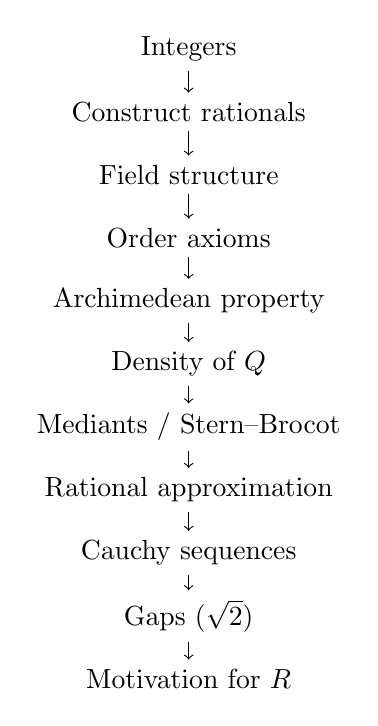
\begin{tikzpicture}[node distance=8mm]

\node (a) {Integers};
\node (b) [below of=a] {Construct rationals};
\node (c) [below of=b] {Field structure};
\node (d) [below of=c] {Order axioms};
\node (e) [below of=d] {Archimedean property};
\node (f) [below of=e] {Density of $\mathbb{Q}$};
\node (g) [below of=f] {Mediants / Stern--Brocot};
\node (h) [below of=g] {Rational approximation};
\node (i) [below of=h] {Cauchy sequences};
\node (j) [below of=i] {Gaps ($\sqrt{2}$)};
\node (k) [below of=j] {Motivation for $\mathbb{R}$};

\draw[->] (a)--(b);
\draw[->] (b)--(c);
\draw[->] (c)--(d);
\draw[->] (d)--(e);
\draw[->] (e)--(f);
\draw[->] (f)--(g);
\draw[->] (g)--(h);
\draw[->] (h)--(i);
\draw[->] (i)--(j);
\draw[->] (j)--(k);

\end{tikzpicture}
\end{center}

This progression reflects the conceptual development of the number
systems used throughout analysis.

\subsection{Construction of the Rational Numbers}

\begin{definition}
Let
\[
W = \mathbb{Z} \times (\mathbb{Z}\setminus\{0\})
\]

and define the relation

\[
(a,b) \sim (c,d) \quad \Longleftrightarrow \quad ad = bc .
\]

The set of rational numbers is defined as

\[
\mathbb{Q} = W / \sim .
\]

An element of $\mathbb{Q}$ is written

\[
\frac{a}{b}.
\]
\end{definition}

This construction formalizes the familiar idea of fractions while ensuring
that different representations of the same number are identified.

\subsection{Field Structure}

\begin{definition}
For $a,b,c,d \in \mathbb{Z}$ with $b,d\neq0$ define

\[
\frac{a}{b}+\frac{c}{d}
=
\frac{ad+bc}{bd}
\]

\[
\frac{a}{b}\cdot\frac{c}{d}
=
\frac{ac}{bd}
\]
\end{definition}

\begin{theorem}
The rational numbers form a field.
\end{theorem}

\subsection{Order Structure}

In addition to their algebraic structure, the rational numbers admit
a natural ordering.

Modern analysis texts often formulate order using the set of
\emph{positive elements}.

\begin{definition}[Positive cone]

Let $P\subset \mathbb{Q}$ be the set of positive numbers satisfying

\begin{enumerate}

\item $P+P \subseteq P$
\item $P\cdot P \subseteq P$
\item For every $a\in\mathbb{Q}$ exactly one holds

\[
a\in P, \qquad a=0, \qquad -a\in P
\]

\end{enumerate}

Define

\[
a<b \iff b-a\in P.
\]

\end{definition}

\subsection{Consequences of the Order Axioms}

\begin{theorem}
For every $a\in\mathbb{Q}$,

\[
a^2 \ge 0.
\]
\end{theorem}

\begin{theorem}
If $a>0$ then $a^{-1}>0$.
\end{theorem}

\begin{theorem}
If $a<b$ and $c>0$ then

\[
ac < bc .
\]
\end{theorem}

\begin{theorem}
If $a<b$ and $c<0$ then

\[
ac > bc .
\]
\end{theorem}

\begin{theorem}
\[
1>0
\]
\end{theorem}

\begin{corollary}

For every natural number $n$,

\[
n>0.
\]

\end{corollary}

\subsection{The Archimedean Property}

\begin{theorem}[Archimedean Property]

For every $x\in\mathbb{Q}$ there exists $n\in\mathbb{N}$ such that

\[
n > x .
\]

\end{theorem}

This property ensures that the integers are unbounded within the rational
numbers.

\subsection{Density of the Rational Numbers}

\begin{theorem}[Density of $\mathbb{Q}$]

For any real numbers $a<b$ there exists a rational number $q$ such that

\[
a < q < b .
\]

\end{theorem}

\begin{proof}

Choose $n$ such that

\[
\frac{1}{n} < b-a .
\]

By the Archimedean property there exists an integer $m$ satisfying

\[
a < \frac{m}{n}.
\]

Then

\[
\frac{m}{n} < a + \frac{1}{n} < b.
\]

Thus

\[
a < \frac{m}{n} < b.
\]

\end{proof}

This theorem shows that rational numbers are everywhere dense on the
number line.

\subsection{Mediants and the Stern--Brocot Tree}

\begin{definition}[Mediant]

For two fractions

\[
\frac{a}{b},\qquad \frac{c}{d}
\]

the mediant is

\[
\frac{a+c}{b+d}.
\]

\end{definition}

\begin{theorem}

If

\[
\frac{a}{b} < \frac{c}{d}
\]

then

\[
\frac{a}{b}
<
\frac{a+c}{b+d}
<
\frac{c}{d}.
\]

\end{theorem}

Repeated mediant construction generates the
\emph{Stern--Brocot tree}, which enumerates every positive rational number
exactly once.

\subsection{Rational Approximation}

The mediant property provides a powerful method for approximating
real numbers by rationals.

\begin{theorem}[Dirichlet Approximation]

For every real number $\alpha$ and integer $N>0$ there exist integers
$p,q$ with

\[
1\le q\le N
\]

such that

\[
\left|\alpha-\frac{p}{q}\right|<\frac{1}{qN}.
\]

\end{theorem}

This theorem reveals that rational numbers approximate real numbers
remarkably well.

\subsection{Cauchy Sequences in $\mathbb{Q}$}

\begin{definition}

A sequence $(q_n)$ of rational numbers is called Cauchy if

\[
|q_m-q_n|<\varepsilon
\]

for all sufficiently large $m,n$.

\end{definition}

Every convergent sequence is Cauchy, but the converse does not hold
in $\mathbb{Q}$.

\subsection{Gaps in the Rational Numbers}

\begin{theorem}

There is no rational number whose square equals $2$.

\end{theorem}

\begin{proof}

Assume

\[
\left(\frac{p}{q}\right)^2 = 2
\]

in lowest terms.

Then

\[
p^2 = 2q^2
\]

so $p$ is even.

Let $p=2k$. Substituting gives

\[
q^2 = 2k^2
\]

so $q$ is also even.

This contradicts the assumption that $p/q$ was reduced.

\end{proof}

Thus $\sqrt{2}$ is not rational.

Nevertheless rational numbers can approximate $\sqrt{2}$ arbitrarily
closely.

\subsection{Motivation for the Real Numbers}

The rational numbers therefore contain \emph{gaps}.
Sequences may converge toward numbers that do not lie in $\mathbb{Q}$.

To remedy this defect we enlarge the number system.

The real numbers can be constructed by

\begin{itemize}

\item Dedekind cuts, or
\item equivalence classes of Cauchy sequences.

\end{itemize}

The resulting system $\mathbb{R}$ is the
\emph{complete Archimedean ordered field}.